
\begin{comment}
TODO: Comentar sobre la naturaleza del sistema que estamos diseñando
-------------------------
El sistema que estamos diseñando es orientado a detección y alerta de fraude sobre transacciones YA REALIZADAS!

NO sobre intentos de transacciones! (preventivo)

Se podría escalar a ello para evitar la realización de transacciones que fuesen detectadas como posibles fraudes, sin embargo esto complicaría la gestión de los filtros ya que:

1. filtro detectaría posible fraude; transacción tentativa quedaría en espera
2. filtro tendría que recibir de vuelta del sistema bancario si al final se autorizó, a pesar de la alerta, esa transacción o no, para poder eliminarla / limpiar el filtro.
Si esto no sucediera así entonces en el caso de que no se autorizara finalmente la transacción tentativa podríamos estar teniendo en el filtro una "falsa transacción" y por tanto estar causando conflictos o generando nuevas alertas que no deberían de estar generándose por culpa de no haber limpiado el filtro de esta transacción no realizada.
-------------------------
\end{comment}

\section{Decoupled Event Handling}

\textcolor{gray}{
In the case of having a shared buffer to communicate the edges between the filter and the worker a mutex is needed. This is because the filter and the worker can possible write and read, respectively, into this buffer at the same time. With it we will avoid race conditions in the sharing of the buffer. However, a channel or other kind of tool would be needed to indicate the worker that there is an edge ready to be read in the buffer. Not having this, would imply to continuosly have the worker requesting the mutex to read from the buffer, even when it is empty and there is no edge to read. 
Therefore as a much more simple alternative, we decided to use an internal channel \texttt{internal\_edge} in between the filter and the worker. With it we avoid having to use a mutex and leading with its derived coordination issues. As a general use case channels are typically used for \emph{passing the ownership of data} which is the case we are dealing with.
}

\section{Multiple Cards Support}

    % Manual control of the size of the map
    To control the maximum number of cards per \filter to the defined \emph{maxFilterSize} value, $|V_{\mathsf{F}}| \leq $ \emph{maxFilterSize}, we needed to control the 
    
    Note that golang maps are inherently dynamic in size. -> control the desired maximum size by ourselves. 

    \textcolor{red}{Issue: "fatal error: concurrent map read and map write"}

    More details -- in Golang it is not defined what happens when we have simultaneous read/write operations:

    \begin{itemize}
      \item \href{https://go.dev/doc/faq#atomic_maps}{Maps Atomicity}
      \item \href{https://go.dev/doc/go1.6}{Runtime. Use of maps}
      \item \href{https://go.dev/blog/maps}{Golang maps. Concurrency}
      \item \href{https://groups.google.com/g/golang-nuts/c/_XHqFejikBg?pli=1}{Golang maps concurrency - blog}
    \end{itemize}

    2 hash tables (to avoid race conditions in concurrent access by filter \& worker):
    \begin{itemize}
      \item \texttt{cardList}: to control the belonging cards to the filter. Only access by filter.
      \item \texttt{cardSubgraph}: to map each belonging card to its corresponding subgraph. Only access by worker.
    \end{itemize}

\section{Communication - Channels}

\item \mathsf{endchan}: synchronization channel between Filter and Worker, to let Filter know whenever Worker is done. To avoid finishing the filter before the worker is actually done. \textcolor{red}{TODO: Include in the drawing}

\section{Old Implementation Details}

\subsubsection{Transaction flux}

\subsubsection{Filter's management and volatile subgraph}

% 0. Qué es. Para qué lo necesito. 
% 1. Cómo es. Data structure description selection
% 2. Cómo funciona. Requisitos funcionales. Descripción funcionamiento.
% * Comentar data structure y operaciones relacionadas: newGraph, update, addAtEnd
% * Tiempo de vida filtro, gestión de esto, eliminación del filtro...

% 0. Qué es. Para qué lo necesito. 
With the purpose of tracking the activity of each of the cards on each of the filters we build a \textit{windowed} volatile subgraph, which has as edges all the transactions belonging to the card that were registered during the last fixed window of time. This volatile subgraph is going to be updated based on the flux of transactions of the pipeline. We need to have this volatile continuously updating subgraph per each of the cards as a \textit{short-term memory} register of the last transactions of a card during a certain window of time, so that whenever a new transaction comes we can make associations/relations with the transactions registered on that last window of time and possibly alert of a potential fraud whenever it is the case.\\
Therefore, the continuous update consists of adding new incoming transactions and discarding the old transactions that fall outside the fixed window of time. This ensures that only transactions inside the fixed window of time are considered to do associations for fraud detection. 
% 1. Cómo es. Data structure description selection
Based on these premises, the data structure to keep the volatile subgraph needs to have two main properties:
\begin{itemize}
    \item Efficient to add new transactions/edges.
    \item Efficient to delete the transactions/edges that are outdated in relation to the fixed \textit{window} of time.
\end{itemize}

Considering that the transactions arrive ordered in time, a linked list was selected as a suitable approach to save the transactions/edges ordered by timestamp. It allows a cheap and easy way to manage the volatile subgraph by adding the new transactions at the tail of the list and deleting the outdated ones from the head of the list. The golang \href{https://pkg.go.dev/container/list}{\texttt{container/list}}, implemented as a doubly linked list was used as an already given implementation of the desired linked list.

\textcolor{cyan}{Another possible alternative considered was the golang \texttt{[] slice} which is a dynamically-sized array. The problem of it was the inefficiency on the deletion from the head of the slice, which had a time complexity of 
$O(n)$, where $n$ is the number of elements in the slice, since it required shifting all the remaining elements to the left.}

Another aspect to consider is the deletion of the filter whenever no transactions related to it are registered after a long period of time. Note that the deletion of the filters after a certain time of inactivity is done due to the huge overhead that it would imply to keep them all simultaneously whenever we are considering a big amount of cards.

The filter's data structure and the operations related to it are described in what follows.

% 2. Cómo funciona. Requisitos funcionales. Descripción funcionamiento.
% * Comentar data structure y operaciones relacionadas: newGraph, update, addAtEnd
% * Tiempo de vida filtro, gestión de esto, eliminación del filtro...
\paragraph{Data Structure}

\begin{center}
\lstset{style=golangStyle}
\begin{lstlisting}[caption={filter subgraph data structure}]
type Graph struct {
	last_timestamp time.Time
	edges          *list.List
}
\end{lstlisting}
\end{center}

The filter inner data structure \texttt{Graph} contains the linked list needed to save the volatile subgraph: \texttt{edges}, which is a linked list of transactions (\texttt{Edge}) belonging to the filter within the fixed window of time (see an example in Figure \ref{img:pipeline-subgraph}), and a timestamp: \texttt{last\_timestamp} which saves the timestamp of the last edge that was added to the filter's subgraph. This is used to check for the deletion of the filter in the case of a long time of \textit{inactivity}.

\begin{center}
\lstset{style=golangStyle}
\begin{lstlisting}[caption={Edge of the volatile subgraph, a transaction belonging to the filter}]
// It is an edge of the volatile subgraph
type Edge struct {
	Number_id string    // Card id
	ATM_id    string    // ATM id
	Tx_id     int64     // transaction id
	Tx_start  time.Time // transaction start date time (DD/MM/YYYY HH:MM:SS)
	Tx_end    time.Time // transaction end date time (DD/MM/YYYY HH:MM:SS)
	Tx_amount float32   // transaction amount
}
\end{lstlisting}
\end{center}

\begin{figure}[H]
    \centering
    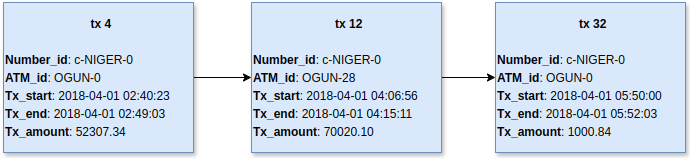
\includegraphics[scale = 0.45]{images/3-Engine/subgraph.png}
    \caption{Subgraph \texttt{edges} linked list of transactions of the \texttt{c-NIGER-0} card filter example}
    \label{img:pipeline-subgraph}
\end{figure}

\paragraph{Operations}
The operations related with the inner filter data structure are the following:

\begin{itemize}
    \item \texttt{NewGraph()}: Creates a new \texttt{Graph} data structure. This is done on the creation of the filter.
    
    \item \texttt{AddAtEnd(e Edge)}: Adds a new edge. Appends a new edge at the end of the list \texttt{edges} and updates the \texttt{last\_timestamp} variable with the \texttt{Tx\_end} time of the new added edge. This operation is done whenever a new transaction edge of the associated card arrives to the filter.
    
    \item \texttt{Update(timestamp time.Time)}: Given a certain datetime, it updates the subgraph, starting from the first edge of the \texttt{edges} list, by eliminating those that are outdated with respect to this datetime. An edge $e$ is outdated  whenever its time difference with respect to the incoming timestamp is greater than the fixed window time constant \texttt{timeTxThreshold}. That is, whenever: $$timestamp - e.Tx\_end \geq timeTxThreshold$$
    This operation is done in two situations:
    \begin{itemize}
        \item $edge \in filter$ ($filter.Number\_id = edge.Number\_id$) Whenever the transaction edge belongs to our filter. Before performing the \texttt{AddAtEnd} operation we perform the \texttt{Update} operation with the timestamp of the new transaction. This ensures that only transactions inside the fixed window of time are considered to do associations for fraud detection. 
        \item $edge \notin filter$ ($filter.Number\_id\ \neq edge.Number\_id$) Whenever a transaction edge passes through our filter but it does not belong to it. We take its timestamp as the \texttt{timestamp} parameter of the \texttt{Update} operation.
    \end{itemize}
    
    \item \texttt{CheckFilterTimeout(timestamp time.Time) bool}: Given a timestamp, it tests if the filter has to be deleted due to a long time of detected \textit{inactivity}. A filter is decided to be deleted if the time difference between the last edge of the subgraph (saved in the \texttt{last\_timestamp} variable) and the incoming \texttt{timestamp} is greater than the fixed \texttt{timeFilterThreshold} time constant: $$timestamp - last\_timestamp \geq timeFilterThreshold$$
    This operation is only performed whenever $edge \notin filter$, taking its timestamp as our parameter, in particular before the \texttt{Update} operation, since in the case the filter needs to be deleted, the \texttt{Update} operation will no longer have to be performed.

    \item \texttt{CheckFraud(new\_e Edge) bool}: \textcolor{blue}{TODO: This is the temporal approximate approach} So far, it is assumed that the current volatile subgraph of the filter is correct (in the sense that it is considered to be free of anomalous transactions). For the moment, only the kind of fraud explained at section \ref{fraud-pattern-1} is checked. \textcolor{blue}{More specifically, the way to perform the check is ONLY between the new incoming edge belonging to the filter \texttt{new\_e} and the last edge that was added to the volatile subgraph. And if, this kind of fraud pattern is matched then an alert is output and this last edge is considered to be anomalous and therefore it is not added to the volatile subgraph of the filter}. 
    
\end{itemize}

With these operations, a summary of the algorithmic behavior of a filter can be seen in the flow diagram on Figure \ref{diag:filter-flow}.

% TODO: Poner ejemplos con dibujitos
% TODO: Diagrama de flujo / casos, para aclarar bien los diferentes casos y qué hago en cada situación
\begin{figure}[H]
    \centering
    \begin{tikzpicture}[node distance=2cm]
\node (start) [startstop] {New Filter (Edge e)};
\node (creation) [process, below of=start] {
    \texttt{NewGraph()}\\
    \texttt{AddAtEnd(e)}
};
\node (while) [process, below of=creation]{in: new edge};
\node (edgeInFilter) [decision, below of=while, yshift=-1cm] {$edge \in filter$};

\node (edgeFilterYes) [process, right of=edgeInFilter, xshift=3cm, text width=4cm] {
    \texttt{Update(edge.Tx\_start)}
    \texttt{AddAtEnd(edge)}
    \texttt{CheckFraud()}
};
\node (filterTimeout) [decision, below of=edgeInFilter, yshift=-2.5cm, text width=3.1cm] {\texttt{CheckFilterTimeout\\(edge.Tx\_start)}};
\node (filterTimeoutNo) [process, right of=filterTimeout, xshift=7cm, text width=4cm] {
    \texttt{Update(edge.Tx\_start)}
};
\node (stop) [startstop, below of=filterTimeout, yshift=-2cm] {Stop};

\draw [arrow] (start) --  (creation);
\draw [arrow] (creation) -- (while);
\draw [arrow] (while) -- node[anchor=east] {edge} (edgeInFilter);
\draw [arrow] (edgeFilterYes) |- (while);
\draw [arrow] (edgeInFilter) -- node[anchor=south] {yes} (edgeFilterYes);
\draw [arrow] (edgeInFilter) -- node[anchor=east] {no} (filterTimeout);
\draw [arrow] (filterTimeout) -- node[anchor=south] {no} (filterTimeoutNo);
\draw [arrow] (filterTimeoutNo) |- (while);
\draw [arrow] (filterTimeout) -- node[anchor=east] {yes} (stop);
\end{tikzpicture}

    \caption{Filter flow diagram}
    \label{diag:filter-flow}
\end{figure}

\paragraph{Considerations}
\begin{itemize}
    \item So far, the way to perform the \texttt{Update} and the \texttt{CheckFilterTimeout} operations could be described as a kind of \textit{filter lazy updating}, since only the filters located before the filter to which the transaction edge finally belongs are updated with the timestamp of that edge. Whereas the filters located after this filter will not be updated with this timestamp. The cause of this is that once the edge is filtered to its corresponding filter, it \textit{sinks} into it, and therefore it is not propagated to the consecutive filters. See the case on Figure \ref{img:pipeline-update-issue}, where if a transaction edge was to belong to the filter F3, then only the filters F1, F2 and F3 will be updated accordingly to the timestamp of this edge, whereas the filter F4 will not be updated in this case.
    \begin{figure}[H]
        \centering
        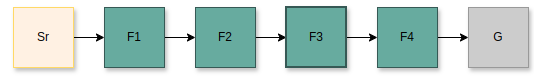
\includegraphics[scale = 0.45]{images/3-Engine/update-issue.png}
        \caption{Pipeline \textit{filter lazy updating} example}
        \label{img:pipeline-update-issue}
    \end{figure}
    However, this is not necessarily a problem. The reason is that the filter will perform these operations later in the future. Note that in the case that the edge belongs to the filter, the \texttt{Update} operation will be performed just before doing the \texttt{AddAtEnd} operation as it was already mentioned in the description of the \texttt{Update} operation. \textcolor{red}{Note that to avoid this "problem" another approach could be done like doing a timestamp channel or passing all the edges until the end of the pipeline.} 
    \item Due to the nature of the management of the filter's lifetime and subgraph updating, it can be the case that our filter subgraph is empty, although the filter is still alive. We can arrive to this situation by having deleted all the edges of the filter subgraph since they were outdated, but still the \texttt{timeFilterThreshold} time has not yet passed. However, thanks to the saved \texttt{last\_timestamp} variable we do not need to save the last edge or do anything but comparing the incoming timestamp with this 
    \texttt{last\_timestamp} variable (calling the function \texttt{CheckFilterTimeout()}).
\end{itemize}
% - last_timestamp parameter helps avoid having to save the last edge completely. The case of the subgraph being empty % but the filter still be active case

% TODO: Tests!!!!
% 1. AddAtEnd -> no añadir...
% 2. Update   -> añadir?
% 3. Filter timeout  -> añadir? (*) igual sólo añadir este, pues es más completo e incluye a los anteriores
\end{graysection}